\section{System Design and Development}
\subsection{Overview}
\begin{figure*}[h]
	\centering
	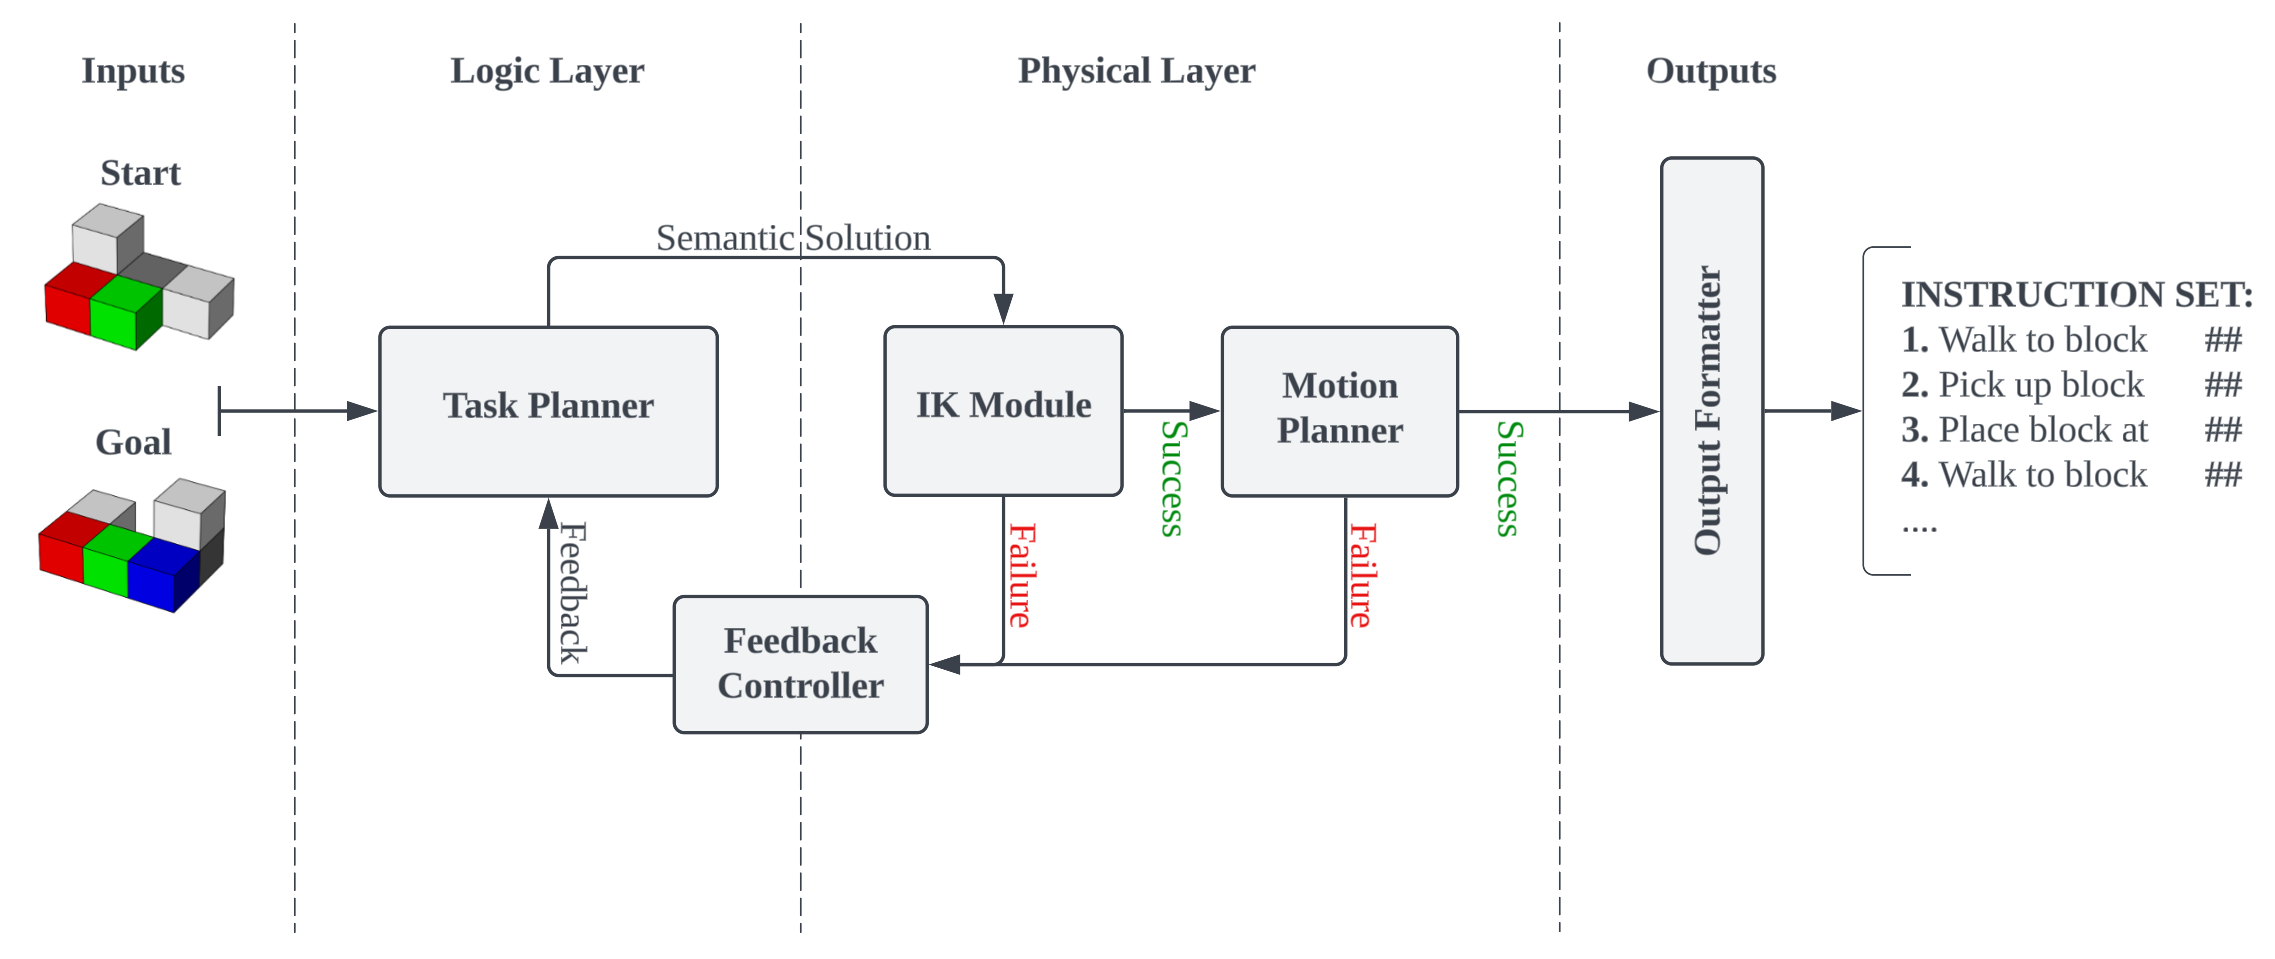
\includegraphics[width=\textwidth]{systemDesign.png}
	\caption{High-level System Design}
	\label{systemDesign}
\end{figure*}

The Reconfiguration Task and Motion Planner (TAMP) program is designed using Python, leveraging existing Python implementations\cite{EVASDK} for controlling the robotic arm \cite{evaSpec} available in the lab. The program inputs an initial and final state and outputs a list of instructions to reconfigure the initial state into the final state using a mobile manipulator.
\\\\
The TAMP system comprises three main components: the logic layer, the physical layer, and the feedback controller. Each component has a distinct role, allowing the discrete and continuous aspects of the solution search to be managed separately while ensuring integration and communication between layers through the feedback controller.
\begin{itemize}[]
	\item\textbf{Logic Layer:} Responsible for discrete task planning.
	\item\textbf{Physical Layer:} Manages continuous motion planning.
	\item\textbf{Feedback Controller:} Integrates the logic and physical layers, facilitating communication and iterative solution searching through feedback strategies.
\end{itemize}
The feedback strategies implemented by the feedback controller create a control loop behaviour, iteratively refining the solution. Once a feasible solution is found, it is formatted into the required instruction set by the output formatter.

\subsection{Logic Layer}
\subsubsection{Overview}
The logic layer of the TAMP program functions as a Task Planner, managing the discrete portion of the search to find semantic solutions. These solutions are sequences of state configurations, each differing by one module movement, that transform the initial state configuration into the goal state configuration.
\\\\
While many contemporary task planners use machine learning techniques to find solutions, these are unsuitable for the space industry due to their black box behaviour. Instead, the TAMP program employs simple graph search techniques to ensure transparency and reliability.

\subsubsection{Searching the Graph}
To search the graph and find the path to the goal state configuration, two major search algorithms are considered: Depth-First Search (DFS) and Breadth-First Search (BFS).
\begin{itemize}[]
	\item\textbf{Depth-First Search (DFS):} In DFS, the algorithm explores a path to its full depth before backtracking and trying alternative paths. This can be implemented using a state priority queue that sorts states based on their proximity to the goal state, enabling quick solutions. However, the resulting path may not be the most efficient for the mobile manipulator, as each state transition involves additional movement.
	\item\textbf{Breadth-First Search (BFS):} In contrast, BFS explores all states at one depth level before proceeding to the next level. It searches all states one step away from the starting state, then two steps away, and so on. Although BFS is much slower than DFS and less scalable to larger numbers of modules, it guarantees finding paths with the fewest transitions to the goal state, making it more suitable for efficient reconfiguration.
\end{itemize}
Given the requirement for solution efficiency over planner speed, the Task Planner implements the BFS algorithm. The pseudo-code for the Task Planner algorithm is shown in Listing \ref{SearchPseudo}.

\begin{lstlisting}[caption={Task Planner search algorithm pseudo-code},captionpos=b,label={SearchPseudo}]
	FIND PATH (S_start, S_goal, max_branches)
	search_tree <- []
	S_current <- S_start
	WHILE S_current NOT S_goal DO
	PriorityQ <- GenNewStates(S_current)
	FOR max_branches DO
	S_new <- PriorityQ.pop(0)
	S_new.parent <- S_current
	search_tree.add(S_new)
	END	
	S_current <- search_tree.pop(0)
	END
	RETURN S_current.GetStatePath()
\end{lstlisting}

\subsubsection{Generating States}
To expand the graph, the task planner generates new states using the \textbf{'GenNewStates()'} function, referenced in the search algorithm pseudo-code (Listing \ref{SearchPseudo}). States are generated based on a set of rules that prioritize which modules to move, ensuring efficient state expansion. The priority rules for module movement are as follows:
\begin{enumerate}[]
	\item Modules not yet in their final position
	\item Modules adjacent to modules not yet in their final position
	\item Remaining modules 
\end{enumerate}
These rules ensure that the task planner consistently generates new states while prioritizing the movement of modules that need to be repositioned first. This approach minimizes unnecessary movements and helps streamline the reconfiguration process.
\\\\
A priority queue that prioritizes modules based on their distance from modules not yet in their final position was considered. This would allow for efficient repositioning of deeply embedded modules. However, this added complexity was deemed unnecessary for the current program's scope and would increase computation time for a relatively rare scenario. For larger structures, implementing such a priority queue could be beneficial to improve computation efficiency.

\subsubsection{Trimming States}
When handling inputs with large numbers of modules, the search tree expansion can quickly result in a vast number of states, consuming significant memory, and computation time. To expedite the search process, generated states are sorted into a priority queue, and only the highest priority states are added to the search graph. The remaining states are discarded, as illustrated in Figure \ref{treeTrimming}. The states are prioritized based on their proximity to the desired goal configuration, using the following heuristics:
\begin{itemize}[]
	\item Number of modules already in their final positions.
	\item Number of modules not in their final positions but occupying positions that are vacant in the goal state.
	\item Sum of the Euclidean distances of the module positions from their final positions in the goal state.
\end{itemize}
These heuristics measure how far a state is from the goal state and allow comparison between states to determine which is closer to the goal. States are first sorted using the number of modules in their final positions. In the event of a tie, the second heuristic is used. If there is still a tie, the computationally intensive third heuristic is applied.
\\\\
By primarily using the first two heuristics, the planner reduces the frequency of expensive calculations, thereby speeding up the state comparison process and improving overall efficiency.
\\\\
\begin{figure*}[h]
	\centering
	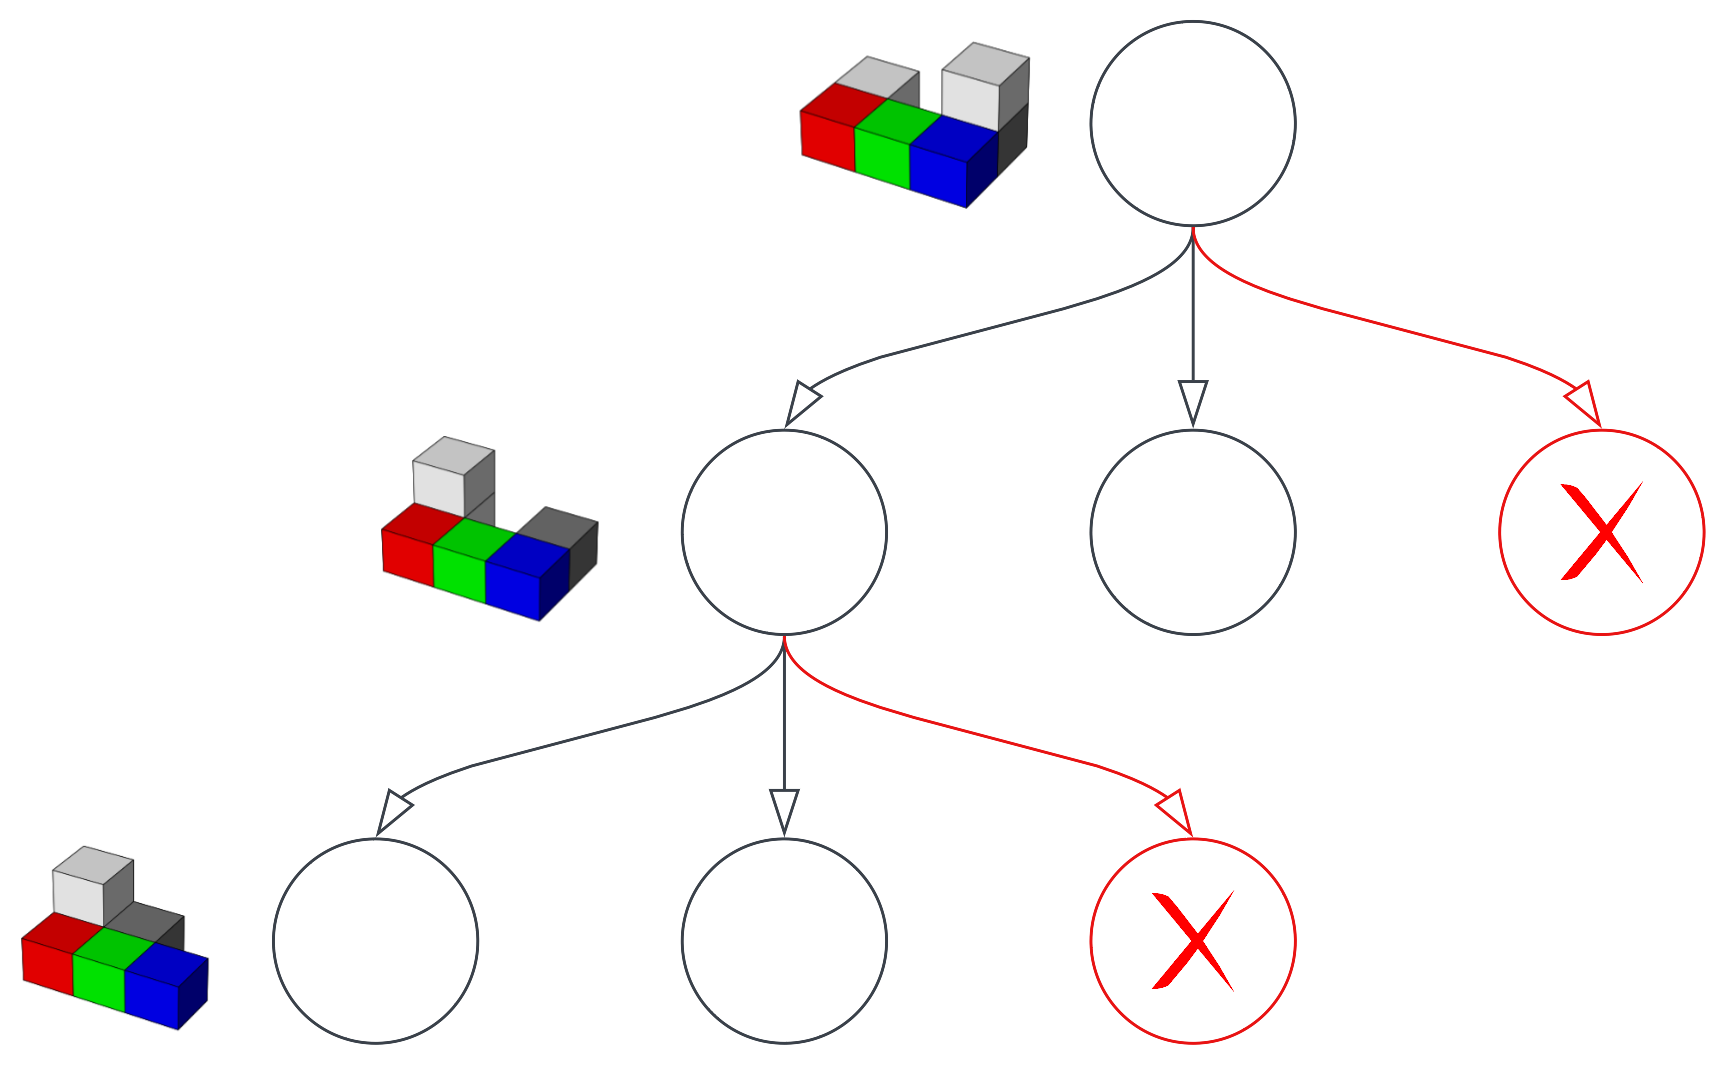
\includegraphics[width=0.7\textwidth]{treeTrimming.png}
	\caption{Selection of generated states demonstration}
	\label{treeTrimming}
\end{figure*}

\subsubsection{Physical Layer Feedback}
When a semantic solution is identified, it is passed to the physical layer for verification. If the physical layer encounters a failure, the transition causing the failure is pruned from the search tree, and all subsequent transitions on that branch are removed. The search then resumes without the failing transition.
\\\\
An alternative approach would involve performing physical layer checks for each move during state generation. However, physical layer calculations are significantly more computationally intensive compared to those in the logic layer. Thus, it is more efficient to focus on verifying only the transitions within the semantic solution, even if it means spending more time searching for these solutions. This approach balances computational load by leveraging the relatively quicker logic layer to identify potential solutions and reserving the intensive checks for validation.

\subsection{Physical Layer}
\subsubsection{Overview}
The physical layer is primarily composed of an inverse kinematics verifier and a motion planner. Its main function is to verify the physical feasibility of transitions in the semantic solution proposed by the logic layer. It processes a semantic solution and returns either a success or a failure.
\begin{itemize}[]
	\item\textbf{Inverse Kinematics Verifier:} This module verifies whether the poses for grabbing and placing a module are possible from the current base position. If either pose is not feasible, the module attempts to find a base position that allows both poses. If both poses are feasible from the same base position, the verifier permits the semantic solution to proceed to the motion planner. If it fails to find such a position, it triggers an inverse kinematics failure and discards the semantic solution.
	
	\item\textbf{Motion Planner:} Upon receiving a transition, the motion planner determines a path from the start pose to the end pose that avoids collisions between the arm, the grabbed module, and other modules. If no collision-free path is found, the motion planner returns a motion planning failure, and discards the semantic solution.
\end{itemize}

\subsubsection{Inverse Kinematics Verifier}\label{IKDESIGN}
Inverse kinematics (IK) determines the joint angles required to position a mobile manipulator's end-effector at a desired location and orientation. There are two primary methods for solving IK \cite{IK}:
\begin{itemize}[]
	\item\textbf{Analytical Approach:} This method involves deriving a mathematical solution specific to each unique manipulator arm. It is complex because it requires detailed analysis and formulation. However, once the formulas are derived, calculations are extremely fast, making it suitable for frequent computations.
	
	\item\textbf{Pseudoinverse Jacobian Method}: This iterative method guesses the required joint angles and adjusts them incrementally to achieve the target position and orientation. It can be applied to any arm configuration without needing unique formulations but is computationally intensive.
\end{itemize}
Given the need for frequent IK calculations, the analytical approach is preferred. The mobile manipulator is represented using Denavit-Hartenberg (DH)\cite{DenavitHartenberg} parameters, which facilitates the derivation of analytical formulae for each joint. The formulae allow for efficient computation of IK, ensuring that the system can quickly verify and adjust the manipulator's poses.

\subsubsection{Manipulator Base Location Planning}
The mobile manipulator present in the MOSAR \cite{MOSAR} project can traverse the modular system. If the IK module fails to connect to a module from a position, moving the arm closer to the module that failed the inverse kinematic check could result in a successful solution like in figure \ref{basePlanning}. When the inverse kinematics module fails a check, it attempts to move the base to another available surface in between the 2 movement points. As our available arm is stationary, our implementation will only include base location planning if time permits.
\begin{figure*}[h]
	\centering
	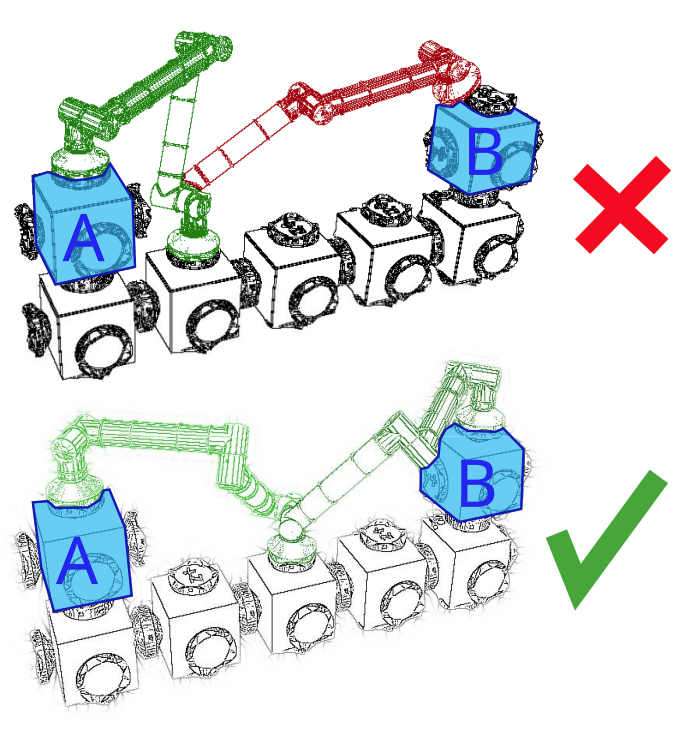
\includegraphics[width=0.5\textwidth]{basePlanning.png}
	\caption{Inverse kinematic checks performed to verify if it is
		possible to translate a module from position A to position B.
		In the first case (above) this is not possible, but it is solved
		by changing the intermediate position in the second case
		(bottom). Image and text from \cite{9438257}}
	\label{basePlanning}
\end{figure*}

\subsubsection{Motion Planning}
Originally, the plan was to implement a motion planner using the Rapidly-exploring Random Tree (RRT) algorithm used here \cite{8412538} to generate collision-free motion paths for the robot arm. However, due to time constraints, a simpler approach is adopted.
\\\\
In the lab scenario, where modules are reconfigured on a platform by a stationary robot arm, motion planning is simplified. We can assume that a module can be picked up if there are no modules above it and if it is within reach according to the inverse kinematic solution. Modules are then moved between positions by lifting them to the arm's maximum z-limit, moving above the new position, and lowering them into place.
\\\\
Additional physical constraints are applied through feedback:
\begin{itemize}[]
	\item Modules cannot be moved to negative-z values due to the platform.
	\item Modules must be placed on top of the platform or another module due to gravity.
\end{itemize}
These constraints will induce physical layer failures, leading to an expected increase in the time taken to generate results compared to operation in space.

\subsubsection{Failure Feedback}
The physical layer reports various types of failures upon detecting conflicts, including:
\begin{itemize}[]
	\item\textbf{Out of reach:} The starting and final positions of the module are unreachable for the current mobile manipulator.
	\item\textbf{No Base Location:} Although the starting and final positions of the module are within reach, there is no suitable base position on the module configuration to reach both points.
	\item\textbf{Collision:} There is no available path to move the module without colliding with another module.
\end{itemize}


\subsection{Feedback Strategies}
Without feedback strategies, the system can find a step-by-step solution to reconfigure modules into the desired goal configuration and verify whether the mobile manipulator can execute the semantic solution. If the mobile manipulator cannot execute the solution, the system fails in its current state.
\\\\
Feedback Strategies establish a control loop that facilitate communication between the logic and physical layers, enabling them to collaborate towards finding solutions that meet their respective goals. While various feedback strategies were considered, the project focuses on implementing those related to final output validation rather than computation time optimization. However, strategies for both aspects were explored in case of early project completion or for future work beyond the project's scope.

\subsubsection{Semantic Solution Verification}
The primary feedback strategy implemented in this project involves simple verification of semantic solutions. Failed solutions are returned to the logic layer, and the problematic transition is removed from the search tree, along with all associated states. The logic layer then continues the search. There is concern that early failures in the physical layer may significantly reduce the search space, potentially hindering the discovery of reasonable solutions. Further testing and research are needed to address this issue and refine the feedback strategy.

\subsubsection{Failure Memory}
Although implementing a failure memory, like the one developed in previous work \cite{9438257}, was considered, it was deemed beyond the project's scope due to its primary focus on time performance. The failure memory utilises a machine learning algorithm to predict physical layer failures based on past data, optimizing the system's runtime by reducing failures. Incorporating a failure memory would provide the system with scalability over time with the collection of failure data, enabling it to generate solutions for larger systems in a reasonable timeframe. Though currently it is unsuitable for space applications due to the reliance on black box machine learning algorithms.  